\chapter{Neural Net Classification Using PCA Derived Filters} \label{appendix:PCAInvestigation}
\myappendices{Appendix \ref{appendix:PCAInvestigation} {Neural Net Classification Using PCA Derived Filters}}
\begin{figure}[htbp] 
  \begin{center}
   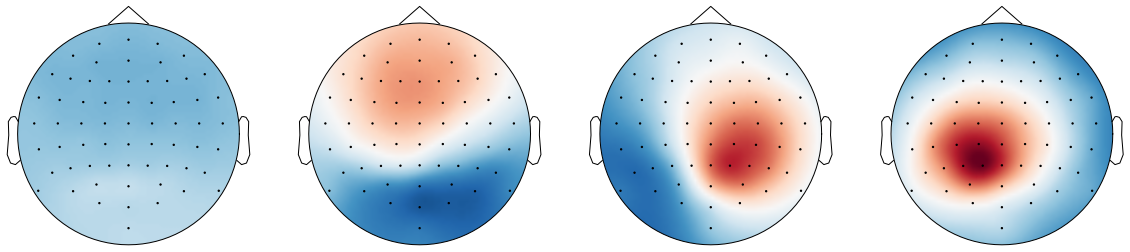
\includegraphics[width=.5\textwidth,keepaspectratio=true]{Figures/PCA_SVM}
   \\\vspace{-0.8em}
    \caption{Principal component analysis (PCA) done on all perception training trials (432 trials)}
    \label{fig:PCA_SVM}
  \end{center}
\end{figure}
\begin{figure}[htbp] 
  \begin{center}
    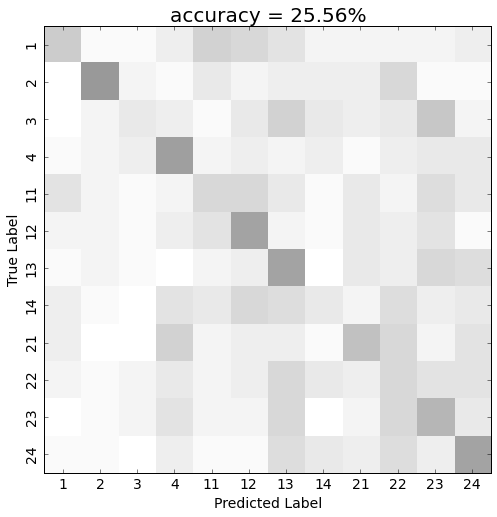
\includegraphics[scale=0.5]{Figures/PC0_confusion}
   \\\vspace{-0.8em}
    \caption{Classification results when layer 1 of the neural net is replaced with the first component from Figure C.1}
    \label{fig:PC0_confusion}
  \end{center}
\end{figure}
\begin{figure}[htbp] 
  \begin{center}
    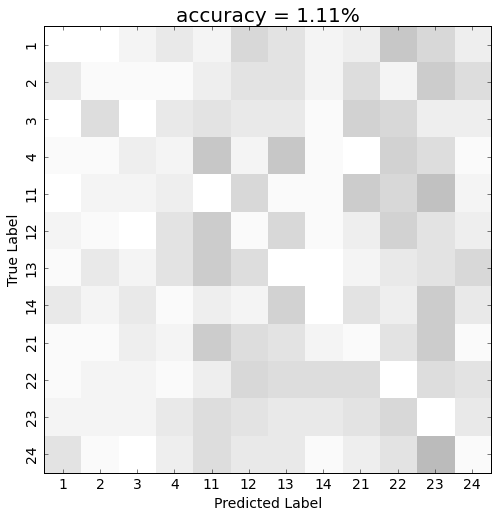
\includegraphics[scale=0.5]{Figures/PC1_confusion}
   \\\vspace{-0.8em}
    \caption{Classification results when layer 1 of the neural net is replaced with the second component from Figure C.1}
    \label{fig:PC1_confusion}
  \end{center}
\end{figure}
\begin{figure}[htbp] 
  \begin{center}
    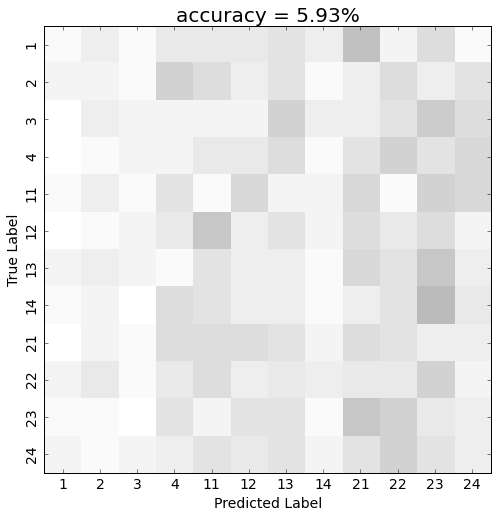
\includegraphics[scale=0.5]{Figures/PC2_confusion}
   \\\vspace{-0.8em}
    \caption{Classification results when layer 1 of the neural net is replaced with the third component from Figure C.1}
    \label{fig:PC2_confusion}
  \end{center}
\end{figure}
\begin{figure}[htbp] 
  \begin{center}
    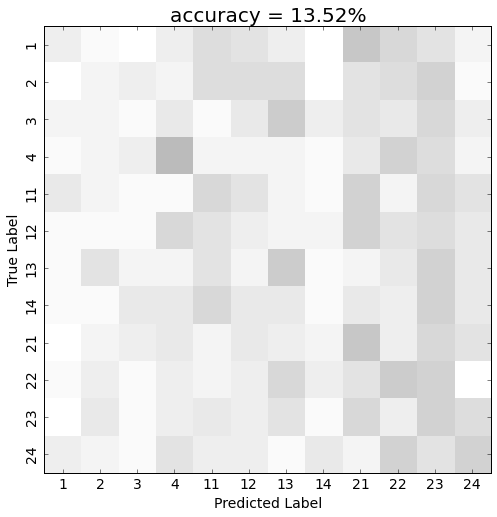
\includegraphics[scale=0.5]{Figures/PC3_confusion}
   \\\vspace{-0.8em}
    \caption{Classification results when layer 1 of the neural net is replaced with the fourth component from Figure C.1}
    \label{fig:PC3_confusion}
  \end{center}
  \vspace{-1em}
\end{figure}